\begin{figure}[htbp]
\section*{ TBX5}
\centering
\begin{subfigure}[b]{0.95\textwidth}
\centering
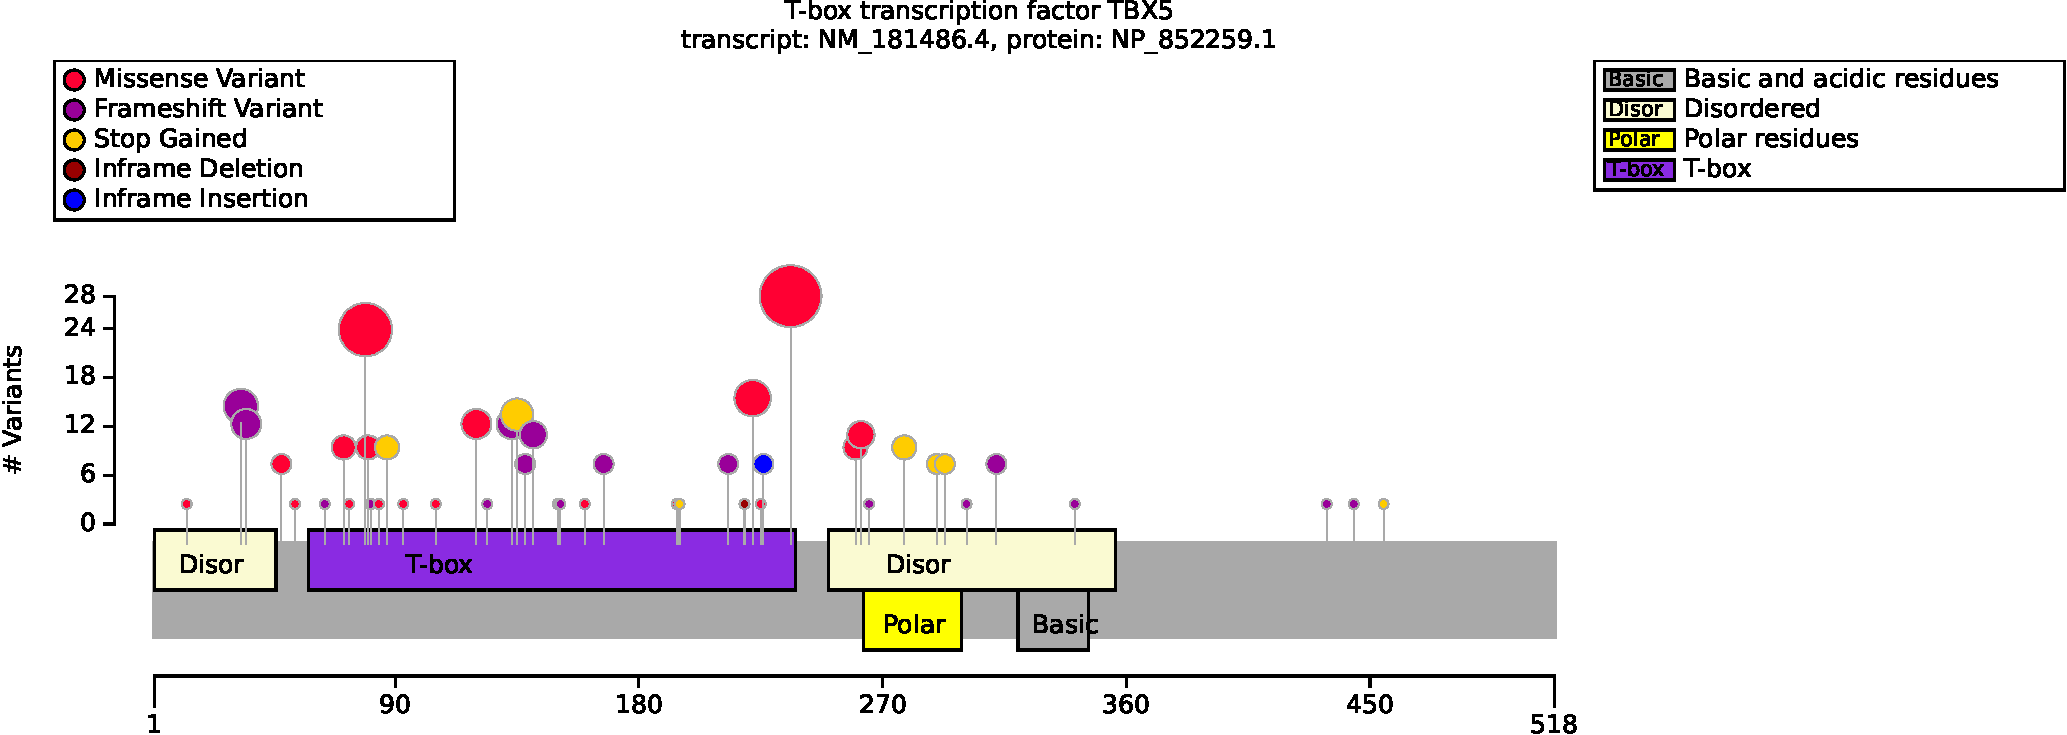
\includegraphics[width=\textwidth]{ img/TBX5_protein_diagram.pdf} 
\captionsetup{justification=raggedright,singlelinecheck=false}
\caption{Distribution of variants in TBX5}
\end{subfigure}

\vspace{2em}

\begin{subfigure}[b]{0.95\textwidth}
\centering
\resizebox{\textwidth}{!}{
\begin{tabular}{llllrr}
\toprule
HPO term & missense & other & p-value & adj. p-value\\
\midrule
Ventricular septal defect [HP:0001629] & 31/60 (52\%) & 30/30 (100\%) & $4.63\times 10^{-7}$ & $8.81\times 10^{-6}$\\
\bottomrule
\end{tabular}
}
\captionsetup{justification=raggedright,singlelinecheck=false}
\caption{Fisher Exact Test performed to compare HPO annotation frequency with respect to missense and other. Total of
        19 tests were performed.}
\end{subfigure}
\vspace{2em}
\begin{subfigure}[b]{0.95\textwidth}
\centering
\resizebox{\textwidth}{!}{
\begin{tabular}{llllrr}
\toprule
HPO term & Arg237Gln & other & p-value & adj. p-value\\
\midrule
Ventricular septal defect [HP:0001629] & 0/17 (0\%) & 61/73 (84\%) & $5.55\times 10^{-11}$ & $1.06\times 10^{-9}$\\
\bottomrule
\end{tabular}
}
\captionsetup{justification=raggedright,singlelinecheck=false}
\caption{Fisher Exact Test performed to compare HPO annotation frequency with respect to Arg237Gln and other. Total of
        19 tests were performed.}
\end{subfigure}
\vspace{2em}
\begin{subfigure}[b]{0.95\textwidth}
\centering
\resizebox{\textwidth}{!}{
\begin{tabular}{llllrr}
\toprule
Genotype (A) & Genotype (B) & total tests performed & significant results\\
\midrule
Gly80Arg & other & 18 & 0\\
FEMALE & MALE & 5 & 0\\
\bottomrule
\end{tabular}
}
\captionsetup{justification=raggedright,singlelinecheck=false}
\caption{Fisher Exact Test performed to compare HPO annotation frequency with respect to genotypes.}
\end{subfigure}

\vspace{2em}

\caption{ The cohort comprised 156 individuals (56 females, 46 males, 54 with unknown sex). 
A total of 90 HPO terms were used to annotate the cohort. Disease diagnosis: Holt-Oram syndrome (OMIM:142900).
Vanlerberghe et al. (2019)] observed that isolated septal CHD are more common in the truncating than in 
the missense variants (p=0.02) \cite{PMID_30552424}.
A total of 156 unique variant alleles were found in \textit{TBX5} (transcript: \texttt{NM\_181486.4}, protein id: \texttt{NP\_852259.1}).}
\end{figure}
